% \title{The Three-Terminal Black Box}
% \author{An Introduction to Physics through Experiments}
% \date{}
% \maketitle

\chapter{The Three-Terminal Black Box}

\section*{Objectives}

\begin{enumerate}
\item To study a three-terminal black box and identify the circuit within it along with the values of the electronic components.

\item To understand the responses of different active and passive circuit elements and their combinations, and learn to recognise them.

\item To exercise your deductive and inductive powers, much as real physicists must do with real experiments.

\end{enumerate}




\section*{Apparatus}

\begin{enumerate}
\item A black box with three connecting terminals marked A, B and C
\item A variable DC power supply (\textit{Keltronix})
\item Two digital multimeters (\textit{MECO 603})
\item A signal generator (\textit{Testronix 72})
\item A Digital Storage Oscilloscope (\textit{GW INSTEK–GDS-1102U})
\item A digital stopwatch (\textit{Racer})
\item A resistor ladder
\item Connecting wires

\end{enumerate}


\section*{Introduction}

You are given a sealed box on which three terminals marked A, B and C are provided which connect to a circuit inside. The circuit inside the box consists of \textbf{three} electronic components of different kinds (i.e. resistors, p-n junction diodes, batteries, etc.). Please note that the black box may consist of combinations of either only one or only two or all three types of components. 

The components may be connected in either a `star' or `delta' connection (refer to the theory section for details). You are expected to identify the interior components as to type and value, and determine how they are connected to each other and to the terminals. 


\section*{Description}

In \textbf{Part A}, the black box will contain only combinations of resistors, p-n junction diodes, and batteries in a \textit{star} connection.

In \textbf{Part B} \textit{(optional)}, the black box will contain only combinations of resistors, p-n junction diodes and capacitors in a \textit{star} connection. 

In \textbf{Part C} \textit{(optional)}, the black box will contain only combinations of resistors, p-n junction diodes, and batteries in a \textit{delta} connection. 

In \textbf{Part D} \textit{(optional)}, the black box will contain only combinations of  resistors, capacitors, and inductors in a \textit{star} connection.


\section*{Theory}

\subsection*{Star and Delta Connections}

Standard 3-component circuits take on two major forms with names that represent the way in which the components are connected: a \textbf{Star} sometimes represented by Y, and a Delta connected network sometimes represented by a triangle or $\Delta$. Both these forms, represented in Figure (\ref{fig:starAndDelta}), are indistinguishable from each other, in that for every star connection there is an equivalent delta connection (with different values for the individual components) and vice versa. It is for this reason that you must keep in mind what form circuit in the black box has before drawing any conclusions.

\begin{figure}[!htb]
       \begin{subfigure}[t]{0.3\textwidth}
				\centering
                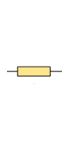
\includegraphics[scale=0.8]{comp.png}
                \captionsetup{justification=centering}
                \caption{Component or combination \\of components}
       \end{subfigure}%
       \begin{subfigure}[t]{0.3\textwidth}
				\centering
                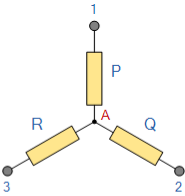
\includegraphics[scale=0.6]{star.png}
                \caption{Star connection}
        \end{subfigure}%
        \begin{subfigure}[t]{0.3\textwidth}
        		\centering
                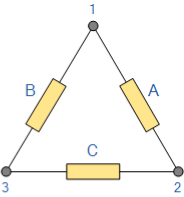
\includegraphics[scale=0.6]{delta.png}
                \caption{Delta connection}
        \end{subfigure}%
        \caption{Circuit connections}
        \label{fig:starAndDelta}
\end{figure}

\begin{figure}[!htb]
\centering
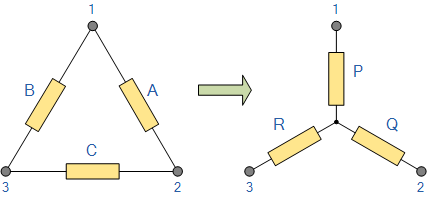
\includegraphics[scale=0.6]{stardelta.png}
\caption{Star to Delta conversion}
\label{fig:starToDelta}
\end{figure}

The following formulae will allow you to move between a star connection and its associated delta connection and vice versa:

\begin{minipage}{0.5\textwidth}
\centering
\paragraph*{Delta to Star Network:}
\begin{equation*}
\begin{aligned}
P &= \frac{A B}{A + B + C}\\
Q &= \frac{A C}{A + B + C}\\
P &= \frac{B C}{A + B + C}\\
\end{aligned}
\end{equation*}
\end{minipage}
\begin{minipage}{0.5\textwidth}
\centering
\paragraph*{Star to Delta Network:}
\begin{equation*}
\begin{aligned}
A &= \frac{P Q + Q R + R P}{R}\\
B &= \frac{P Q + Q R + R P}{Q}\\
C &= \frac{P Q + Q R + R P}{P}\\
\end{aligned}
\end{equation*}

\end{minipage}


\subsection*{Passive circuit components}

Passive circuit components are electrical components that cannot control the current in a circuit. They do not generate power, but instead dissipate, store, and/or release it. Some such components are discussed below.

\subsubsection*{Resistors}

A resistor is a two-terminal passive electronics component used to oppose or limit the current in a circuit. A resistor works based on the principle of Ohm’s law which states that the voltage applied across the terminals of a resistor is directly proportional to the current flowing through it, with the constant of proportionality called the \textit{resistance}.

\begin{equation*}
V = I R
\end{equation*}

\subsubsection*{Capacitors}

A capacitor, made from two conductive plates with an insulator between them, stores electrical energy in the form of an electric field. It blocks the DC signals and allows the AC signals to pass through it. The charge stored in a capacitor is given by

\begin{equation*}
Q = CV
\end{equation*}

When used with a resistor, the time a capacitor takes to charge or discharge is measured in units of an intrinsic time scale, known as the time constant $\tau = RC$ of the circuit.

\subsection*{Active circuit components}
An active device is any type of circuit component with the ability to electrically control electron flow in the circuit.

\subsubsection*{Batteries}

Charges can be separated by several means to produce a voltage. A battery uses a chemical reaction to produce energy and separate opposite sign charges onto its two terminals. As the charge is drawn off by an external circuit, doing work and finally returning to the opposite terminal, more chemicals in the battery react to restore the charge difference and the voltage.


\subsubsection*{p-n junction Diodes}

A p-n junction diode is two-terminal semiconductor device, which allows the electric current in only one direction while blocks the electric current in opposite or reverse direction. Such a diode has an anode (or positive end) containing positive charge carriers called `holes', and a cathode (or negative end) containing negative charge carriers or electrons. The interface between these ends forms a region without any charge carriers called the \textbf{depletion layer}. 

The process of applying the external voltage to a p-n junction semiconductor diode is called biasing. If the diode is \textbf{forward biased} -- that is, when a positive voltage is applied to the anode and a negative voltage to the cathode -- it allows the charge carriers, and hence electric current, to flow. On the other hand, if the diode is \textbf{reverse biased} -- negative to the anode and positive to the cathode -- it blocks the current flow. In the conventional symbol for a diode, the arrowhead indicates the conventional direction of electric current when the diode is forward biased.

Unlike a resistor, a diode does not behave linearly with respect to the applied voltage as the diode has an exponential current-voltage (I-V) relationship and therefore cannot be described by simply using an equation such as Ohm’s law. The basic reason for this is that the width of the depletion layer decreases with increase in positive voltage. After a certain `knee' voltage (0.3 V for Germanium semiconductors and 0.7V for Silicon semiconductors) the width of the barrier effectively goes to zero, and the diode acts like a short circuit with zero resistance. When a junction diode is reverse biased the thickness of the depletion region increases and the diode acts like an open circuit blocking any current flow (except only a very small leakage current), until an `avalanche' voltage when the device overheats and gets shorted leading again to maximum current flow in the opposite direction.

\begin{figure}[!htb]
\centering
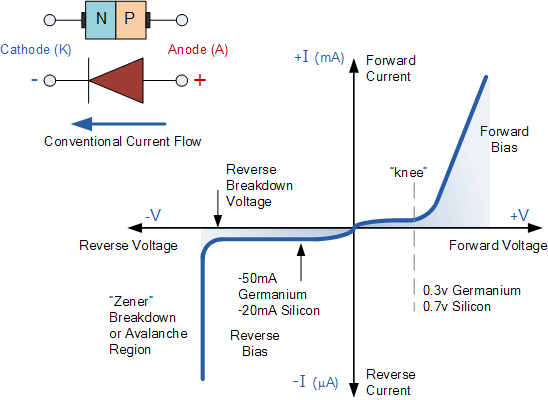
\includegraphics[scale=0.6]{diodeChar.png}
\caption{Diodes and their characteristics}
\label{fig:diodeChar}
\end{figure}



\section*{Experimental Setup}


\subsection*{Black Box}
The black box contains an unknown circuit inside it which is connected to terminals A, B, and C in either a `star' or a `delta' connection (explained above). You have to use these for your analysis and measurements. Do not try to open the given black box.

\subsection*{Digital Multimeter (\textit{MECO 603})}

A multimeter is an instrument used to measure multiple parameters like voltage, current, and resistance. In this experiment you will use the given digital multimeters (Model \textit{MECO - 603}) \textbf{\textit{only}} for the measurement of DC and AC voltage and current. You will have to use input sockets marked COM, V/$\Omega$ and mA (or 20A) for the required measurements. Note that there are two input sockets marked mA and 20A for the current measurement. The socket marked mA may be used for measuring current below 250 mA and socket marked 20A may be used for measuring current up to 20 A. You will have to select the appropriate function and the range using the rotary switch provided on the multimeter. The value of voltage or current is displayed on the LCD screen. The multimeter is turned off by turning the dial to the appropriate setting.

\subsection*{Variable DC Power Supply (\textit{Keltronix})}

The power switch can be used to switch it ON or OFF. The required output can be taken from the two output terminals. The voltage and the current capacity can be changed using the three knobs: voltage coarse, voltage fine, and current. The given power supply also displays the value sof the output voltage and current. Do not use these value since measuring these values using given calibrated multimeter will be more reliable. 

The DC Variable Power Supply can either act as a source of Constant Current (CC) or Constant Voltage (CV), indicated by the two LEDs present on it. In general, most types of circuits require a constant voltage to operate, so if the CV LED is lit, the supply is working fine with your circuit. The power supply has a physical limit on how much current it can supply, if the load (your circuit) attempts to draw more, the power supply decreases the output voltage to keep the current consumed at its maximum permissible amount. For this experiment, you should turn the current dial up to the maximum. This allows the supply to work as a constant voltage supply unless the current drawn by your circuit goes beyond 1A.

\subsection*{Function Generator (\textit{Testronix 72})}

A function generator is a type of signal generator that is used to generate simple repetitive waveforms in the form of an alternating electrical wave. Typically, it will produce waveforms or functions such as sine waves, sawtooth waveforms, square, and triangular waveforms, and will allow you to adjust the frequency and amplitude of  the signals. The instrument given to you generates sine and square waveforms. The output may be taken from the output sockets for the respective waveforms. The frequency can be adjusted by turning the dial and selecting the appropriate Frequency Multiplier button. For example, turning the dial to 3 and selecting the 10k button would provide an output waveform with a frequency of 30kHz. Similarly the amplitude switch, used in conjunction with the appropriate buttons, can be used to adjust the amplitude of the output waveform from under 0V to 30V.



\subsection*{Warnings}

\begin{enumerate}
\item The use of a multimeter to measure the resistance is strictly prohibited.
\item Do not try to open the black box, use only terminals A, B and C for the connections.
\item Use fixed value resistors to prevent large currents in the circuit. The current should not exceed 500 mA.
\item \textbf{Do not} short the outputs of the power supply, it could damage the equipment.
\item Passing more current through the multimeter's (250 mA or 20A) sockets than they can handle will cause the fuses in the multimeter to burn out, leading to an open circuit. Use an appropriate resistance to limit the current in the circuit.
\item When drawing circuit diagrams use the standard symbols.
\item The digital multimeter, the DC power supply or the signal generator should be turned off if not in use.

\end{enumerate}


\section*{Procedural Instructions}

Design the most appropriate method to identify the circuit and determine the values of the electronic components used  in it. Give your answer in the form of a circuit diagram showing the terminals A, B, and C clearly. You will need to give \textit{all} the information required in order to reconstruct the circuit. For example, if you are doing Part A, you will need to determine the values of the resistors, the orientation of the diodes, and the voltage and orientation of the battery, if any of the above are used in the circuit.

In every part, clearly report the procedural steps you have taken with reference to your complete plan of experiment, the data will you collect, how the collected data will be analysed and finally the interpretation of your analysis. Your reporting should be comprehensive, and you are expected to mention all important procedural steps in your answer sheet.



\section*{References}

\begin{enumerate}

\item \href{https://www.elprocus.com/major-electronic-components/}{Overview of Various Basic Electronics Components}

\item \href{https://www.electronics-tutorials.ws/dccircuits/dcp_10.html}{Star Delta Transformation}

\item \href{https://www.electronics-tutorials.ws/diode/diode_3.html}{Electronics Tutorials: PN Junction Diode}

\end{enumerate}


\newpage